\chapter{Corrosion Classification}
\section{Extreme environments}
We study the influence of slow and fast chemistry on structures. Mediated through chemistry that occurs on the surface of materials. This is generally through electrochemical processes that are generally associated with corrosion. Corrosion covers a vast area of material science so we must first go through some of the key electrochemical processes which we cover in this lecture. We are generally interested in the long term view.
\section{Corrosion}
Corrosion is defined as the conversion of metal to a more chemically stable form by chemical and / or electrochemical reaction with their environment. Metals are susceptible because they are good conductors. Corrosion degrades the useful properties of material and structures including strength.
\subsection{Corrosion is similar to a battery}
\begin{figure}[H]
    \centering
    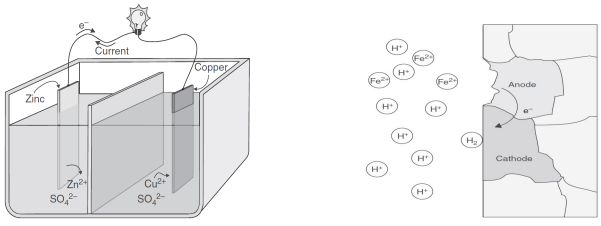
\includegraphics[width = 0.8 \textwidth]{img/figure70.png}
    \caption{Corrosion mechanism compared to battery.}
\end{figure}
This requires an exchange and so only occurs when there are differences. This is classified as either:
\begin{enumerate}
    \item Two different metals in the same liquid
    \item Two different liquids with the same metal
\end{enumerate}
To understand how to stop corrosion, we will have two choices - either coat materials or understand why reaction occurs. First step is to understand the basics of electrochemistry - chemistry is an exchange of electrons. If something is oxidised then something else must be reduced. Reactivity depends what is in the aqueous mixture in contact with the metal.
\subsection{Electrode potentials}
\begin{figure}[H]
    \centering
    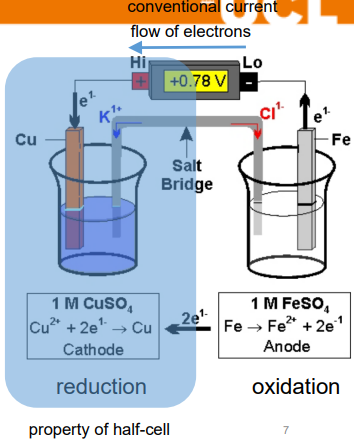
\includegraphics[width = 0.5 \textwidth]{img/figure71.png}
    \caption{Copper reduction and iron oxidation setup in galvanic cell.}
    \label{copperRedIronOx}
\end{figure}
If the iron and copper electrodes are connected electrically, reduction will occur for copper at the expense of the oxidation of iron. \ce{Cu^2+} ions will deposit (electrodeposit) as metallic copper on the copper electrode, while iron dissolves (corrodes) on the other side of the cell and goes into solution.
\begin{align}
    \ce{Fe -> Fe^2+ + 2e^-} \qquad       & \textrm{(oxidation)}        \\
    \ce{Cu^2+ + 2e^- -> Cu} \qquad       & \textrm{(reduction)}        \\
    \ce{Cu^2+ + Fe -> Cu + Fe^2+} \qquad & \textrm{(overall reaction)}
\end{align}
\subsection{Salt bridge}
A salt bridge is used to connect the oxidation and reduction half-cells of a galvanic cell (voltaic cell), a type of electrochemical cell. It maintains electrical neutrality within the internal circuit, preventing the cell from reaction. Salt bridges usually come in two types:
\begin{enumerate}
    \item Glass tube - U-shaped glass tube filled with a relatively inert electrolyte; usually potassium chloride or sodium chloride is used (agar is often used as a gelification agent), although Figure \ref{copperRedIronOx} here illustrates the use of a potassium nitrate solution. The conductivity of the glass tube bridge depends mostly on the concentration of the electrolyte solution. An increase in concentration below saturation increases conductivity. Beyond-saturation electrolyte content and narrow tube diameter may both lower conductivity
    \item Filter paper - the other type of salt bridge consists of filter paper, also soaked with a relatively inert electrolyte, usually potassium chloride or sodium chloride because they are chemically inert. No gelification agent is required as the filter paper provides a solid medium for conduction. Conductivity of this kind of salt bridge depends on a number of factors: the concentration of the electrolyte solution, the texture of the filter paper and the absorbing ability of the filter paper. Generally smoother texture and higher absorbency equates to higher conductivity
\end{enumerate}
\subsection{Electrochemical considerations}
\subsubsection{Oxidation reaction}
Metal atoms characteristically lose or give up electrons in what is called an oxidation reaction.
\begin{equation}
    \ce{M -> M^n+ + ne^-}
\end{equation}
where \ce{n} is valence (number of valent electrons). the site at which oxidation takes place is called the anode. Oxidation is sometimes called an anodic reaction. Example:
\begin{gather}
    \ce{Fe(s) -> Fe^2+(aq) + 2e^-}\\
    \ce{Al(s) -> Al^3+(aq) + 3e^-}
\end{gather}
\subsubsection{Reduction reaction}
The electrons from each oxidised metal atom must be transferred to and become a part of another chemical species in what is termed a reduction reaction. In acid solutions, which have a high concentration of hydrogen ions:
\begin{equation}
    \ce{2H^+ + 2e^- -> H2(g)}
\end{equation}
pH = $- \log_{10}\left[\ce{H^+}\right]$, where more \ce{H^+} results in pH $<$ 7. For an acid solution having dissolved oxygen:
\begin{equation}
    \ce{O2 + 4H^+ + 4e^- -> 2H2O}
\end{equation}
For a neutral or basic aqueous solution in which oxygen is dissolved:
\begin{equation}
    \ce{O2 + 2H2O + 4e^- -> 4OH^-}
\end{equation}
Any metal ions present in the solution may be reduced:
\begin{gather}
    \ce{M^n+ + ne^- -> M}
\end{gather}
The location at which reduction occurs is called the cathode. It is possible for two or more of the reduction reactions to occur simultaneously.
\subsection{Galvanic couple}
Two metals electrically connected in a liquid electrolyte wherein one metal becomes an anode and corrodes while the other acts as a cathode.

The question is which one corrodes. An electric potential or voltage will exist between the two cell halves, and its magnitude can be determined if a voltmeter is connected in the external circuit. Various electrode pairs have different voltages; the magnitude of such a voltage may be thought of as representing the driving force for the electrochemical oxidation-reduction reaction.
\begin{align}
    \ce{Cu^2+ + Fe -> Cu + Fe^2+} \quad & \left(\SI{0.780}{\volt}\right) \\
    \ce{Fe^2+ + Zn -> Fe + Zn^2+} \quad & \left(\SI{0.323}{\volt}\right)
\end{align}
Standard half cell: a half-cell of a metal electrode immersed in a \ce{1M} solution of ions and at \SI{25}{\degree C}. To understand reaction, we have to look at one half of the electrochemical cell or half-battery, specifically when one half of the battery is a standard form.
\section{Standard hydrogen reference probe}
It consists of an inert platinum electrode in a \ce{1M} solution of \ce{H^+} ions, saturated with hydrogen gas that is bubble through the solution at a pressure of \SI{1}{atm} and a temperature of \SI{25}{\degree C}.

\textbf{Standard electromotive force (emf) series.} It is generated by coupling to the standard hydrogen electrode, standard half-cells for various metals and ranking them according to the measured voltage. This tells us the potential for reaction but not the rate.
\begin{figure}[H]
    \centering
    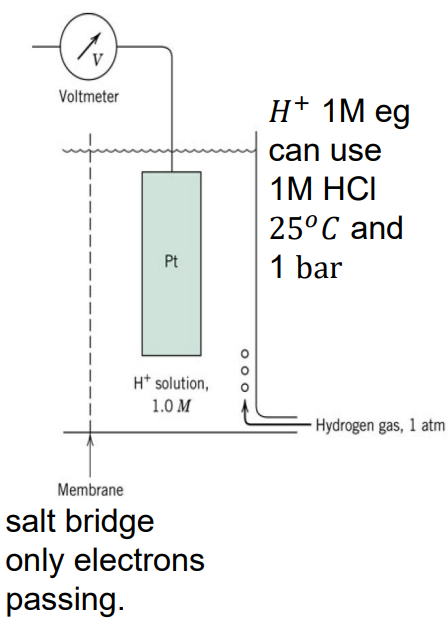
\includegraphics[width = 0.5 \textwidth]{img/figure72.png}
    \caption{Standard hydrogen reference probe.}
\end{figure}
\subsection{Standard emf series}
\begin{table}[H]
    \centering
    \begin{tabular}{@{}lll@{}}
        \toprule
                            & \textbf{Electrode reaction}    & \textbf{Standard electrode}           \\
                            & \textbf{(reduction)}           & \textbf{potential} $V^0$ (\si{\volt}) \\
        \midrule
        Reduction (cathode) & \ce{Au^3+ + 3e^- -> Au}        & +1.420                                \\
                            & \ce{O_s + 4H^+ + 4e^- -> 2H2O} & +1.229                                \\
                            & \ce{Pt^2+ + 2e^- -> Pt}        & +1.200                                \\
                            & \ce{Fe^3+ + e^- -> Fe^2+}      & +0.771                                \\
                            & \ce{Cu^2+ + 2e^- -> Cu}        & +0.340                                \\
                            & \ce{Fe^2+ + 2e^- -> Fe}        & -0.440                                \\
                            & \ce{Zn^2+ + 2e^- -> Zn}        & -0.763                                \\
                            & \ce{Na^+ + e^- -> Na}          & -2.714                                \\
        Oxidation (anode)   & \ce{K^+ + e^- -> K}            & -2.924                                \\
        \bottomrule
    \end{tabular}
    \caption{Table to show standard emf series. Increasingly inert to increasingly reactive from top to bottom. E.g. With \ce{Cu} and \ce{Fe}, \ce{Fe} corrodes. With \ce{Fe} and \ce{Zn}, \ce{Zn} corrodes.}
\end{table}
\section{Classification of corrosion types}
\begin{figure}[H]
    \centering
    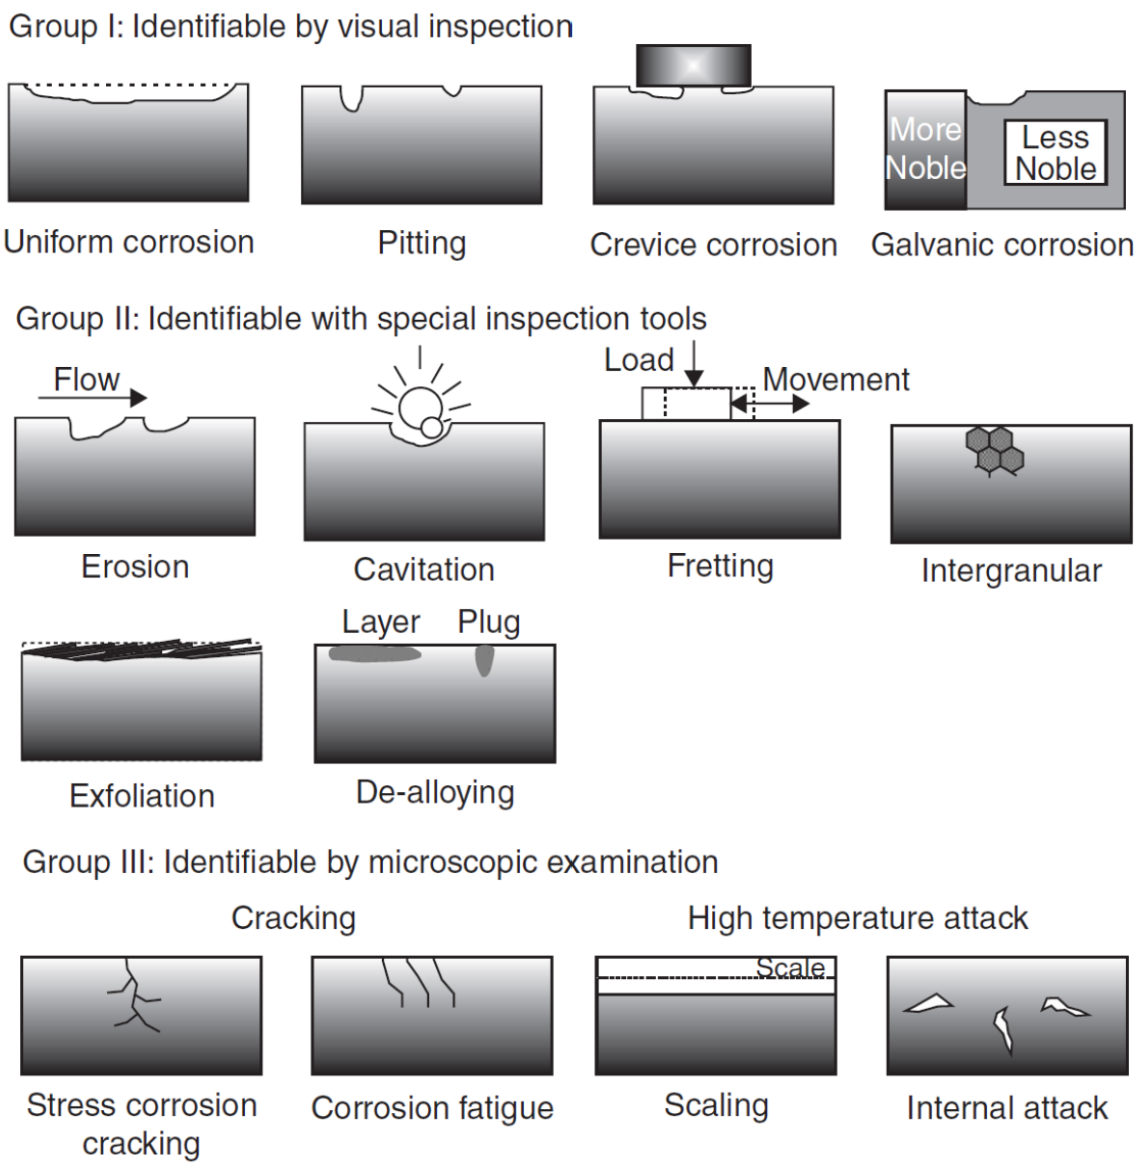
\includegraphics[width = \textwidth]{img/figure73.png}
    \caption{Classification of corrosion types.}
\end{figure}
\subsection{Group 1: corrosion you can see}
\begin{enumerate}
    \item Uniform corrosion characterised by even, regular loss of metal from corroding surface
    \item Localised corrosion during which most of metal loss occurs at discrete areas. This includes crevice corrosion, pitting
    \item Galvanic corrosion occasioned by electrical contact between dissimilar conductors in an electrolyte
\end{enumerate}
\subsection{Group 2: multiple mechanisms}
\begin{enumerate}
    \item Erosion - corrosion. Usually high speed flow with particles, cavitation with bubbles near walls, friction and fretting
    \item Intergranular corrosion at grain boundaries in the metal structure (grains acts a bit like local galvanic couples). Common occurrence which is called weld decay
    \item Dealloying corrosion (selecting leaching) due to selective dissolution of one component of an alloy (e.g. zinc from brass alloy with \ce{O2} and moisture, iron from cast iron)
\end{enumerate}
\subsection{Group 3: microscope corrosion viewed by microscope}
\begin{enumerate}
    \item Corrosion fatigue. Small cracks are enlarged by corrosion and fatigue which then affects the crack growth. Tensile stresses propagate the crack. Corrosion further deteriorate crack
    \item High-temperature corrosion (scaling, internal attack, oxygen corrosion of nickel)
    \item Microbial effects caused by certain bacteria when their metabolism created corrosive elements and deposits. Sulfate-reducing bacteria
\end{enumerate}
\begin{figure}[H]
    \centering
    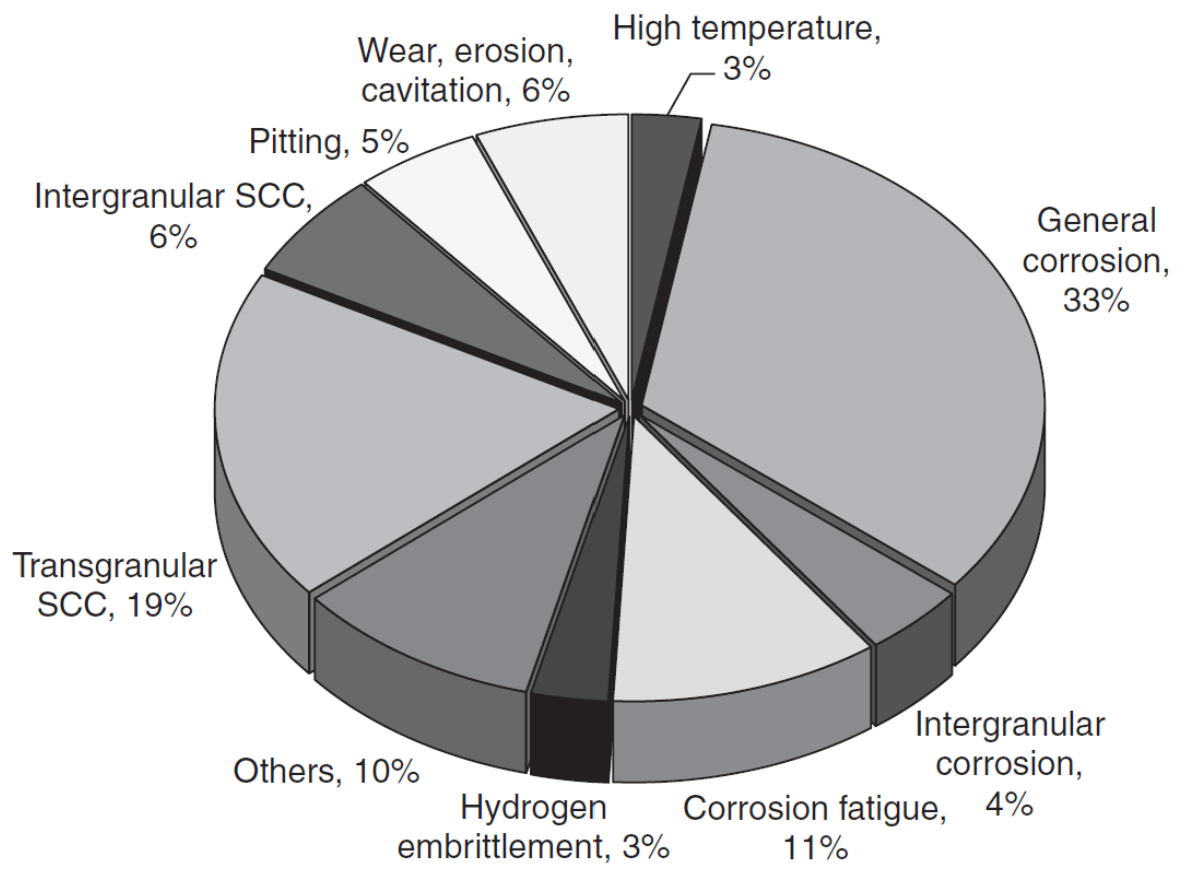
\includegraphics[width = \textwidth]{img/figure74.png}
    \caption{Frequency of different corrosion types.}
\end{figure}
\section{Corrosion mechanisms in-depth}
\subsection{Pitting corrosion}
Creation of small holes in materials which can perforate thin sheets. This is an example of where there is one metal but two types of electrolyte in the vicinity of the metal. This is because the reaction within the hole or pit is not the same as the reaction outside. Pitting results when a small hole or cavity forms in the metal, usually as a result of de-passivation of a small area. This area becomes anodic, while part of the remaining metal becomes cathodic, producing a localised galvanic reaction. The deterioration of this small area penetrates the metal and can lead to failure. This form of corrosion is often difficult to detect due to the fact that it is usually relatively small and may be covered and hidden by corrosion-produced compounds.

Certain conditions, such as low concentrations of oxygen or high concentrations of chloride which complete as anions, can interfere with a given alloy's ability to re-form a passivating film. Corrosion at these points will be greatly amplified, and can cause corrosion pits of several types, depending upon conditions. While the corrosion pits only nucleate under fairly extreme circumstances, they can continue to grow even when conditions return to normal, since the interior of a pit is naturally deprived of oxygen and locally the pH decreases to very low values and the corrosion rate increases due to an autocatalytic process. In extreme cases, the sharp tips of extremely long and narrow corrosion pits can cause stress concentration to the point that otherwise tough alloys can shatter; a thin firm pierced by an invisibly small hole can hide a thumb sized pit from view. These problems care especially dangerous because they are difficult to detect before a part or structure fails. Pitting remains among the most common and damaging forms of corrosion in passivated alloys, but it can be prevented by control of the alloy's environment.

Pitting is autocatalytic in nature. Once a pit starts to grow, the conditions developed are such that further pit growth is promoted. The anodic and cathodic electrochemical reactions that comprise corrosion separate spatially during pitting. The local pit environment becomes depleted in cathodic reactant (e.g. oxygen), which shifts most of the cathodic reaction to the boldly exposed surface where this reactant is more plentiful. The pit environment becomes enriched in metal cations and an anionic species such as chloride, which electromigrates into the put to maintain charge neutrality by balancing the charge associated with the cation concentration. The pH in the pit is lower owing to cation hydrolysis.
\begin{enumerate}
    \item The formation of anodic sits by disruption of the protective passive film on the metal surface.
          \begin{equation}
              \ce{M -> M^n+ + ne^-}
          \end{equation}
          This is balanced by the cathodic reaction of oxygen on the adjacent surface
          \begin{equation}
              \ce{O2 + 2H2O + 4e^- -> 4OH^-}
          \end{equation}
    \item Due to the continuing metal dissolution, an excess of positive ions (\ce{M^n+}) is accumulated in the anodic area. The process is self-stimulating and self-propagating. To maintain charge neutrality negative ions (anions), like chloride, migrate from electrolyte (for example, seawater of a 5\% \ce{NaCl} solution).
          \begin{equation}
              \ce{M^+Cl^- + H2O -> MOH + H^+Cl^-}
          \end{equation}
          \ce{OH^-} ions also migrate to neutralise the positive charges. This process is called hydrolysis
    \item The presence of (\ce{H^+}) ions and chloride content, prevents repassivation. The above the process generates free acid and the pH value at the bottom of pit is substantially lowered (1.5-1.0)
    \item The increase in the rate of dissolution at the anode increases the rate of migration of the chloride ions and the reaction becomes time dependent and continues, resulting in the formation of more and more \ce{M^+Cl^-}, generation of more and more \ce{H^+Cl^-} by hydrolysis
    \item The process continues until the metal is perforated. The process is autocatalytic and it increases with time resulting in more and more dissolution
    \item Finally, the metal is perforated and the reaction is terminated
\end{enumerate}
\begin{figure}[H]
    \centering
    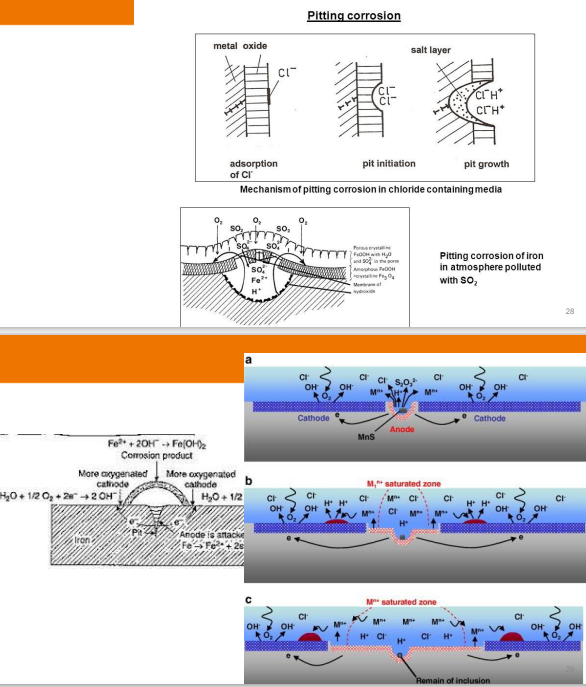
\includegraphics[width = \textwidth]{img/figure75.png}
    \caption{Pitting corrosion.}
\end{figure}
\subsection{Crevice corrosion}
Crevice corrosion is a localised form of corrosion occurring in confined spaces (crevices), to which the access of the working fluid from the environment is limited. Formation of a differential aeration cells leads to corrosion inside the crevices. Examples of crevices are gaps and contact areas between parts, under gaskets or seals, inside cracks and seams, spaces filled with deposits and under sludge pile.

Crevice corrosion is influenced by the crevice type (metal-metal, metal-non-metal), crevice geometry (size, surface finish) and metallurgical and environmental factors. The susceptibility to crevice corrosion can be evaluated with ASTM standard procedures. A critical crevice corrosion temperature is commonly used to rank a material's resistance to crevice corrosion.
\subsubsection{Mechanism}
\begin{figure}[H]
    \centering
    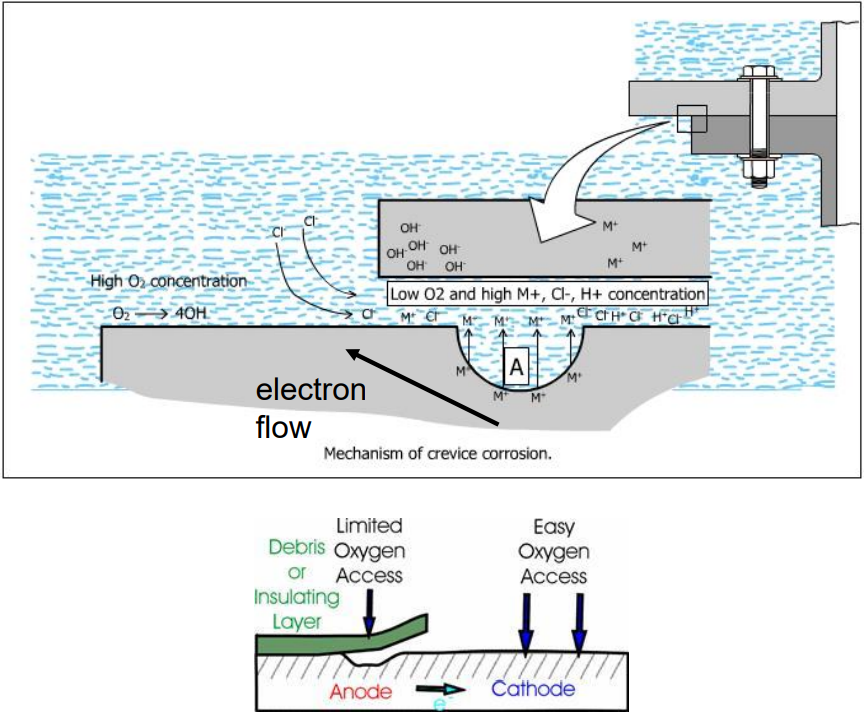
\includegraphics[width = 0.8\textwidth]{img/figure76.png}
    \caption{Mechanism of crevice corrosion.}
\end{figure}
Crevice corrosion is initiated by a difference between some chemical constituents, usually oxygen, which sets up an electrochemical concentration cell. Outside of the crevice (the cathode), the oxygen content and pH are higher - but chlorides are lower.

Chlorides concentrate inside the crevice (the anode) worsening the situation. Ferrous ions forms ferric chloride and attack the stainless steel rapidly. The pH and oxygen content are lower inside the crevice (can be as low as 2). Once the crevice has formed the propagation mechanism continues.
\begin{figure}[H]
    \centering
    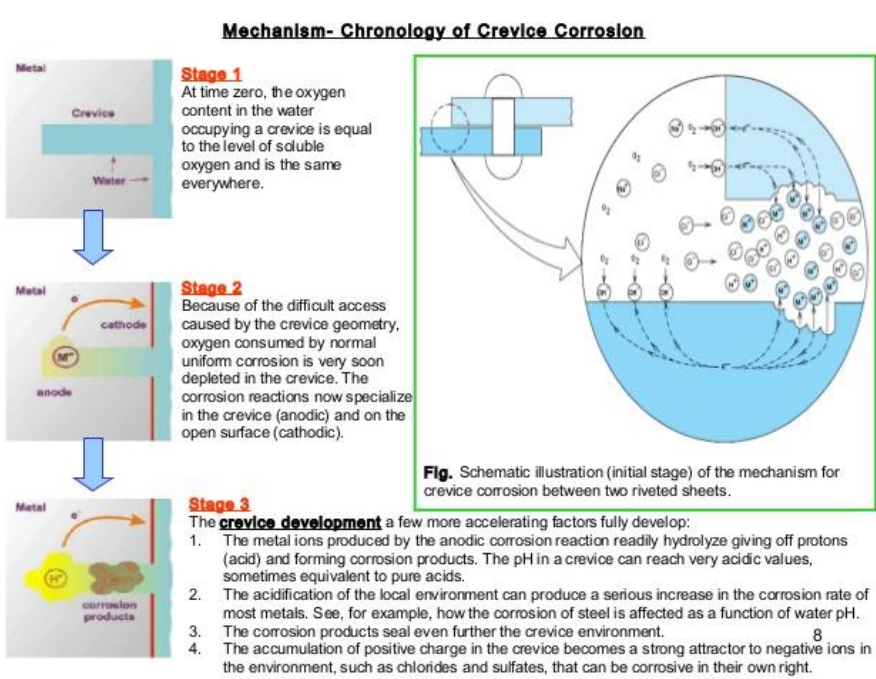
\includegraphics[width = 0.8\textwidth]{img/figure77.png}
    \caption{Chronology of crevice corrosion.}
\end{figure}